%%%%%%%%%%%%%%%%%%%%%%%%%%%%%% -*- Mode: Latex -*- %%%%%%%%%%%%%%%%%%%%%%%%%%%%
%% 09-02.tex --     ESEM 2009 Submission
%% Author          : Philip Johnson
%% Created On      : Wed Jan 07 14:06:37 2009
%% Last Modified By: Philip Johnson
%% Last Modified On: Wed Aug 05 12:12:27 2009
%% RCS: $Id$
%%%%%%%%%%%%%%%%%%%%%%%%%%%%%%%%%%%%%%%%%%%%%%%%%%%%%%%%%%%%%%%%%%%%%%%%%%%%%%%
%%   Copyright (C) 2009 
%%%%%%%%%%%%%%%%%%%%%%%%%%%%%%%%%%%%%%%%%%%%%%%%%%%%%%%%%%%%%%%%%%%%%%%%%%%%%%%
%% 

\documentclass[times,10pt,twocolumn]{article} 
\usepackage{latex8}
\usepackage{times}
\usepackage{graphicx}

\begin{document}

\pagestyle{empty}

\title{We need more coverage, stat!  \\
Classroom experience with the Software ICU}

\author{
Philip Johnson\\
Shaoxuan Zhang \\
Collaborative Software Development Laboratory\\
Department of Information and Computer Sciences\\
University of Hawaii\\
}


\maketitle
\begin{abstract}
For empirical software engineering to reach its fullest potential, we must
develop effective, experiential approaches to learning about it in a
classroom setting.  In this paper, we report on a case study involving a
new approach to classroom-based empirical software engineering called the
``Software ICU''.  In this approach, students learn about nine empirical
project ``vital signs'' and use the Hackystat Framework to put their
projects into a virtual ``intensive care unit'' where these vital signs can
be assessed and monitored.  We used both questionnaire and log data to gain
insight into the strengths and weaknesses of this approach. Our evaluation
provides both quantitative and qualitative evidence concerning the overhead
of the system; the relative utility of different vital signs; the frequency
of use; and the perceived appropriateness outside of the classroom
setting. In addition to benefits, we found evidence of measurement
dysfunction induced directly by the presence of the Software ICU. We
compare these results to case studies we performed in 2003 and 2006 using
the Hackystat Framework but not the Software ICU.  We use these findings to
orient future research on empirical software engineering both inside and
outside of the classroom.
\end{abstract}

%% One goal of the Hackystat Framework is to investigate novel approaches to
%% teaching software measurement in classroom settings, and we evaluated one
%% such approach in 2003 \cite{csdl2-03-12} and another in 2006
%% \cite{csdl2-07-02}.  This paper describes our most recent approach called
%% the ``Software ICU''.

%\category{D.2.8}{Software Engineering}{Metrics}[complexity measures, performance measures, software quality measures]

\Section{Introduction}

Introducing students to software measurement in particular and empirical
software engineering in general is a challenging task.  

On the one hand, if one merely lectures about the literature, much of the
subtleties involved in the practice of collecting and analyzing process and
product data are lost.  An overly superficial presentation can lead
students to believe that empirical software engineering is ``easy''. For example,
simply (1) collect complexity; (2) set a threshold using a published
reference such as \cite{Clark08}, and (3) require developers to ``fix'' any
classes that exceed the established threshold.  The problem is that
individual metrics never capture the spectrum of trade-offs implicit in a
design. For example, a natural result of performance optimization on a
section of code is an increase in complexity (and coupling). Measurements
on such classes might exceed thresholds for important reasons.  Without
such real world grounding, such students could grow up to be the
stereotypical process improvement managers who impose ``best practices''
for measurement and analysis without understanding the potential for
misinterpretation and, ultimately, measurement dysfunction \cite{Austin96}.

On the other hand, requiring students to gather and analyze measurements
themselves can potentially lead students to believe that empirical software
engineering is too ``hard''.  For example, while the Personal Software
Process \cite{Humphrey95} provides a well structured approach to data
gathering and analysis by students, independent research reveals a number
of problems including high overhead \cite{csdl2-01-12}, data quality
\cite{csdl-98-13}, and low adoption \cite{Borstler02}.  Students introduced
to metrics via the PSP (or its successor, the Team Software Process) can
easily form the impression that empirical approaches impose too much
overhead for (at the very least) ``agile'' software development situations.

For the past five years, one research thrust of the Hackystat Framework has
been to explore the issues involved in teaching empirical software
engineering in a classroom setting \cite{csdl2-03-12,csdl2-07-02}.
Hackystat provides a pedagogical middle ground between excessively high
overhead approaches like the PSP/TSP and excessively low overhead
approaches like literature review.  Extensive automation of both data
collection and analysis lowers the overhead required to give students
practical experience with measurement, while creating opportunities to
understand some of the nuances involved with analysis, presentation, and
interpretation.

In this paper, we present the results of a case study experiment we
performed in the Fall of 2008 in which we used the metaphor of a medical
intensive care unit (ICU) to explain and motivate the use of empirical
software engineering.  We built a new user interface for empirical data called
the ``Software ICU'' that is similar in many ways to a medical ICU
monitoring device.  Just as a medical ICU automatically gathers vital signs
of patients such as heart rate and respiration in order to detect changes
in health, our software ICU automatically monitors the process and product
``vital signs'' of its software ``patients''---in this case, the student
teams and the projects they were developing.  Just as a medical ICU
generates alarms when a vital sign falls outside a established range for
normalcy, the software ICU can color metrics as red, yellow, or green to
indicate problematic, unstable, or healthy software vital signs.

We collected two types of data: an on-line questionnaire that the students
filled out at the end of the study, and system-generated log data that
collected all student interactions with the Software ICU.  Our results
provide evidence that, in general, the Software ICU is the most effective
Hackystat-based approach to teaching students about process and product
measurement.  Student feedback indicates that the overhead involved in data
collection and analysis was acceptably low, and almost all of the students
found the data to be useful, although students found some ``vital signs''
to be more useful than others. Most students believed that the Software ICU
would be feasible for use in professional situations.  The log data
provided independent confirmation of the usage of the system, as the
majority of students invoked the Software ICU from 20 to 40 times per week
during the course of the study.  On the negative side, we found direct
evidence of measurement dysfunction in one student, who was motivated by the
system to engage in behavior counter-productive to the team.

The remainder of the paper is organized as follows.  Section
\ref{sec:related} presents related work.  Section \ref{sec:icu} provides a
brief overview of the system. Section \ref{sec:evaluation} presents the
case study design and its results, followed by a discussion of these results
in Section \ref{sec:discussion}.   Section \ref{sec:conclusions} summarizes the 
contributions of this research and some proposed future directions.

\Section {Related Work}
\label{sec:related}

Perhaps the most extensively studied curriculum for measure\-ment-based
software engineering is the Personal Software Process \cite{Humphrey95} and
the Team Software Process \cite{Humphrey00}.  Both of these approaches
require students to develop a series of software projects, typically six to
eight during a single semester.  Both process and product measures are
gathered about each project, and the measurements become increasingly
detailed as the semester proceeds. After the first three projects are
completed, the students can use the completed projects as historical data
to support quality improvement (by identifying repeated types of defects)
and estimation (through simple linear regression).  The PSP/TSP methods
enjoy strong support from the Software Engineering Institute, and they have
a published a number of case studies indicating success in a classroom setting. 

Conn developed a metrics-based software engineering course called the 
IS Integrated Capstone Project \cite{Conn04}.  The metrics were closely aligned
with the PSP/TSP format, though some of the process constraints were relaxed. 

PSP/TSP approaches require a significant amount of manual data
collection and analysis due to the nature of the analyses of interest. In
prior research \cite{csdl2-00-03}, we implemented extensive tool support
for PSP/TSP style of data collection and analysis, but still found the
overhead to be substantial \cite{csdl2-01-12}. In contrast, the Software ICU provides
significantly more automation of data collection and analysis, but focuses
on different kinds of data collection and analyses than the TSP/PSP.

Robillard designed a project-based course in which students were required
to fill out logs that specified the time spent on various activities
\cite{Robillard98}.  However, no automation of data collection was supported in this
approach. 

Two recent research efforts focus on automated data collection to support
introductory programming courses.  Project ClockIt provides automated
facilities for collection of time, compilation attempts and successes, and
size in lines of code based upon a custom plug-in to the BlueJ IDE
\cite{Norris08, Barry05}.  Retina collects similar data on beginning
programmers, although it is enhanced with recommendation and suggestion
features \cite{Murphy09}.  Retina can notice, for example, when a student
is getting many more errors per compilation than other students in the
class, and recommend that the student might want to break the work down
into smaller pieces.

Project ClockIt and Retina are designed around the needs of introductory
programming classes, where students typically work alone, do not use a wide
range of development tools, and a significant amount of energy is devoted
to obtaining a syntactically correct program.  The Software ICU is oriented
to the needs of advanced undergraduate and graduate level software
engineering courses, where team dynamics become significant, compilation is
no longer a significant issue, and a much wider range of tools are employed 
during the course of development.  

There are a great number of commercial toolkits that provide ``dashboards''
for software project data, such as the the LightHouse project management
system, the ProjectManager.com dashboard, the SPMN Project Control Panel,
and so forth. The Software ICU is, of course, one example of a project
dashboard. However, it tends to differ from commercial approaches with
respect to its metrics, user interface, adherence to the medical ICU
metaphor, application to a classroom setting, automated data collection,
and open source development and distribution.  Most importantly, commercial
dashboard organizations have not, to our knowledge, published negative
results regarding their use. Our research contributes new understanding by
providing evidence not only regarding the benefits, but also regarding the potential
negative impact of this class of systems.

The metaphor of ``software health'' is not unique to this research.
Organizations concerned with expensive, life-critical hardware-software
systems have long been concerned with assessing their health at run-time
and potentially recovering from unhealthy states \cite{Hadden00,
Thai01}. Our approach focuses on the health of the system during
development, not execution.

The research presented in this paper is the third case study we have
performed on measurement collection and analysis in a classroom setting
using Hackystat.  In 2003, we performed our first case study in which we used an
early version of Hackystat to automate data collection and analysis and
used a survey to assess student reactions \cite{csdl2-03-12}.  In this
study, we found that students encountered significant problems during the
installation of the system, that analyses were somewhat useful, and that
privacy and platform issues were thought to be significant issues in a
professional setting.

In 2006, we performed a partial replication of the first case study
\cite{csdl2-07-02}.  It was a partial replication because the Hackystat
system had significantly evolved since 2003 and so we changed some of the
evaluation questions to better suit the current needs.  On the positive
side, students reported less problems during installation, reflecting the
work we had done since 2003 on a client-side installer.  On the negative
side, the much larger set of analyses available in 2006 impacted on the
usability of the system: students were more confused about which analyses
to use and how to interpret the results.

For these and other reasons, we decided in 2007 to begin a major
re-implementation of Hackystat as a service-oriented architecture
\cite{csdl2-09-07}. The new system provided us with the ability to redesign
the user interface to Hackystat.  Instead of a single, monolithic user
interface with a predefined look and feel, the new architecture allowed us
to implement multiple, special purpose interfaces using a wide variety of
UI technologies.  

In 2008, we finished the re-implementation of the basic facilities as well
as a new approach to multi-project metrics visualization called Portfolio
Analysis.  In Fall of 2008, we performed a third case study. This time, we
used the metaphor of the ``Software ICU'', as discussed next.

\Section{From Medical to Software ICU}
\label{sec:icu}

Medical intensive care units feature automatic and continuous monitoring of
patient vital signs.  The four fundamental medical vital signs are
temperature, heart rate, blood pressure and respiration.  Other vital signs
may be monitored depending upon the particulars of a patient condition.

\begin{figure}[ht]
  \center
  \includegraphics[width=0.4\textwidth]{micu-screen.eps}
  \caption{An example Medical ICU monitoring device}
  \label{fig:micu}
\end{figure} 

Figure \ref{fig:micu} illustrates a sample medical ICU display unit. For
each of the four fundamental vital signs, the interface shows both its
current numeric value as well as a graph showing its recent history.  

Each of these vital signs has a ``normal range of behavior'', and the
monitoring unit can raise an alarm when any of the patient's vital signs departs
from its normal range of behavior.

Vital signs are interesting because: (a) in a healthy patient, they are
normal or improving; (b) change in one vital sign may or may not be
significant; (c) change in multiple vital signs is almost certainly
significant, particularly if more than one are outside their normal range.

Translating medical ICU practices to the context of a software engineering
class required us to redefine health, vital signs, normal range
and the ICU monitoring user interface into terms useful to students and their
software development projects.

We defined a healthy development project as satisfying three high-level
characteristics: high efficiency (software development proceeds ``as fast
as possible, but no faster''); high effectiveness (effort is focused on the
most important issues, with minimal rework); and high quality (software
satisfies user needs; software can be easily installed, adapted, and
maintained).

We then presented a set of simple practices that, if followed, we claimed
would improve the health of their projects.  These
included: everyone works consistently; everyone contributes equally; code
is committed consistently; progress is regular; quality remains high; no
last minute rush to finish.  These development practices are analogous to
life-style behaviors like ``eat right'', ``get enough sleep'' and
``exercise regularly'' that generally facilitate (but, of course, do not
guarantee) good health in a patient.

Next, we presented nine software vital signs: coverage, complexity,
coupling, churn, builds, commits, unit tests, size, and dev
time. Through a combination of Hackystat sensors and the Hudson continuous
integration system, these nine vital signs could be automatically and
continuously collected for their projects.

For each software vital sign, we then presented its normal range of
behavior.  For example, for the coupling vital sign to be considered
healthy, its current value should be above 90\% and the trend in
coverage over time should be stable or increasing.  For the commit vital
sign to be considered normal, at least 50\% of the team members should have
committed, and there should be commits on at least 50\% of the days in the
project interval.  For one of the vital signs, size, we stated that
there is no simple way of assessing its normal range of behavior, though
it still provides some value in understanding project health.

Unlike a medical ICU, where there is literally hundreds of years of medical
research establishing both the importance of the four fundamental vital
signs and their normal range of behaviors, no such consensus exists in
software engineering on what would constitute ``fundamental'' software
vital signs or their normal range of behavior.  Thus, our selection of
software vital signs and their normal range of behaviors are actually
research hypotheses.  We designed the case study to elicit evidence
regarding the appropriateness of these vital signs and our proposed normal
range of behaviors.

Finally, we presented the user interface to the Software ICU. A portion of
this user interface appears in Figure \ref{fig:sicu}.

\begin{figure*}[ht]
  \center
  \includegraphics[width=0.8\textwidth]{portfolio-2008.eps}
  \caption{An example Software ICU display}
  \label{fig:sicu}
\end{figure*} 

Each row in the Software ICU interface provides information about one
software project.  Each column presents information about
one vital sign. Similar to the medical ICU, the software ICU presents both
the most recent numeric value as well as the recent trend in value for each
vital sign.

We decided to represent normal range in behavior by independently
coloring the trend line and the most recent value as green, yellow, or red
depending upon whether the value was healthy, unstable, or
unhealthy.  We did not implement alarms, such as emails or text
messages to team members if a vital sign turns red, although this is a
possible future extension.  Instead, it was the responsibility of the
students to invoke the software ICU regularly in order to monitor the
health of their project.  During the case study, we collected log data to
gather evidence about whether they in fact did this monitoring.

To help make the vital sign actionable, the Software ICU supports drill
down for trend data.  Figure \ref{fig:telemetry} shows one such drill-down
that reveals that only one of the four members of the project was doing the
vast majority of commits.

\begin{figure*}[ht]
  \center
  \includegraphics[width=0.8\textwidth]{telemetry-screen.eps}
  \caption{A drill-down showing commit telemetry}
  \label{fig:telemetry}
\end{figure*} 

The measurements underlying the Software ICU were collected automatically
through two mechanisms. First, the students installed Hackystat sensors
into their IDE (Eclipse) and build system (Ant) which sent process
metrics regarding their development activities.  Second, their projects
used the Hudson system to perform continuous integration, which meant that
after each commit of their code, the system would be automatically built
and tested.  The Hudson system was also configured to automatically gather
certain product metrics such as coverage, coupling, and complexity.

\Section{Evaluation}
\label{sec:evaluation}

Our case study was focused on addressing the following research questions: 
\begin{itemize}
\item What are the strengths and weaknesses of the medical ICU metaphor for 
teaching software measurement in a classroom setting? 
\item How appropriate were our choices of ``vital signs''?
\item How effective were our algorithms for coloring the vital signs? 
\item How does this approach compare to previous uses of Hackystat to teach software metrics
in a classroom setting? 
\end{itemize}

The study involved 18 students from a senior-level undergraduate software
engineering course at the University of Hawaii from Fall, 2008. This course
teaches software engineering in the context of open source development
using the Java programming language.  The first several weeks are concerned
with basic tools and technologies, including interactive development
environments, coding standards, static analysis tools for quality
assurance, build systems, configuration management, and software review.
The course taught these concepts in the context of a semester project,
which in this semester was a web application for automated tracking and
notification of library book due dates.  We introduced the Software ICU
during the final four weeks of the semester, and the students used it for
two increments of development.

During the final week of the semester, we made available to them an on-line
survey containing 17 questions.  These questions asked the students their
opinions regarding the overhead involved with installing sensors, problems
they encountered, frequency of use of the system, the vital signs they
found useful, and the utility of the system and its appropriateness for an
industrial setting.  A companion technical report to this paper provides
the full text of the survey \cite{csdl2-09-03}.

Students picked a piece of paper from a hat which contained a random six
character ID string.  They provided their chosen ID string and their name
to a graduate student researcher while the instructor was out of the room.
Students used this ID to identify themselves when filling out the on-line
questionnaire.  They were told that the instructor for the class would not
know their responses, but that the graduate student would use the ID on the
completed questionnaires to provide the instructor with a list of students
who had completed the questionnaire.  All students completing the
questionnaire would receive extra credit for participation.  This approach
incentivized participation, provided some level of anonymity to the
students, prevented non-students from completing the survey, prevented
multiple responses by a single student, and allowed the graduate student to
compare the log data for that student to their survey responses in order to
cross-validate some of their answers. All but one of the students in the
class completed the questionnaire.

For complete details on the responses and our analysis of the results, we 
refer you to the companion technical report \cite{csdl2-09-03}.  Space limitations 
require us to present only selected findings. 

\SubSection{Overhead of installation and use}

Automated collection of process and product data cannot be totally free:
there is some effort required to download, install, and configure the
sensors responsible for monitoring developer behavior and the state of the
system.  The first seven questions gathered data about the perceived
overhead of sensor installation and use, as well as requests for details on
problems experienced. The data indicates that Eclipse sensor installation
was very easy for almost all of the students, while installation of sensors
based on the Ant build tool were somewhat more complicated. The most
problematic sensor for students to use successfully was the sensor for
Subversion.  Overhead of use was mixed: one response was {\em ``The sensors ran
automatically and it was fast with sending the data,''} while another was
{\em ``Sending sensor data was often quite slow.''}  

\SubSection{Privacy}

One important impact of the Software ICU is an increase in transparency:
the Software ICU makes it very clear when one or more members of a team are
not contributing.  To find out their views on this issue, we asked the
students how they felt about sharing their software development data with
other members of the class.  Fifteen out of eighteen responses were
generally positive about this aspect, with comments such as, {\em ``I had
no problem with this, and it encouraged me to be aware of my time
management and coding style''.}  One student responded somewhat ironically:
{\em ``Did not really like it because it is showing my programming habits,
like starting on a project in the last couple of days.''}  The most
positive response included the following: {\em ``All group projects in all
schools (e.g. Architecture) should be required to use such a system.''}  On
the other hand, the most negative response included this disturbing
commentary: {\em ``Actually Hackystat (or hacky-stalk as what my teammates
and I called it) caused a lot of arguments and trash talk.  Some guys were
more concerned about collecting stats on Hackystat than actually finishing
the project.''}

\SubSection{Frequency of use}

Two questions asked students to provide a rough sense for how frequently
they used the Software ICU analysis as well as the associated Telemetry
drill-down.  One student said they used it only once a week, while the
remainder were split roughly evenly between ``2-3 times a week'' and
``every day or more''.  We were able to corroborate the students
self-reported frequency of use by examining the log data.  The log data
also revealed that Telemetry was primarily used to look at member-level
data; in other words, while the Software ICU chart would show only
aggregate levels, the Telemetry would show trends on a per-member basis.

\SubSection{Vital signs}

The Software ICU provided data on nine vital signs, and one question listed
them and requested that students check all of them that they found useful.
The DevTime vital sign was checked by every single respondent, and the
Coverage vital sign was checked by all but one.  The remaining vital signs
that more than half of the students found useful were: Commit, Test, Build,
Churn, and Complexity.  Two vital signs were found useful by less than half of the
respondents: Coupling and Size.

One of our central research questions concerned the effectiveness of our
colorization scheme for vital signs, so we asked students whether they felt
the coloring of vital signs accurately reflected their project's health.
Ten of the students responded affirmatively, four of the students responded
negatively, and four effectively responded with ``it depends''.  Some of
the responses revealed insight into the limitations of metrics, such as
{\em ``I felt most of the colors accurately represented the health of the
project. For the coverage data, since we can write test cases just to
increase the [percentage], we cannot assume that the project is in a
healthy condition even if [coverage is green]. However, I think this is not
a problem of Hackystat.''}  Another respondent wrote: {\em ``The ICU was
accurate with our project because it showed drastic spikes in all signs.
This reflects our project in poor health.''}  One of the negative responses
included comments on how pursuing high coverage as an end in itself could
be a waste of time, that DevTime does not measure the time spent reading a
book, and that complexity and coupling are hard to evaluate.

Even if the vital sign colors were accurate, there is still the question of
whether the Software ICU provides actionable information. To assess this,
we asked the students if they were able to use the Software ICU to improve
their software's quality and/or their team's process.  14 students
responded affirmatively, 2 students said it did not, and 1 student was not
sure.  Many of the responses indicated that the member-level drill downs
helped in project management, such as {\em ``We can check how other members
are doing for the project through the Software ICU and this helps a lot
especially when we are working on the team project.''}.  Another student
wrote, {\em ``I think for sure the Software ICU improves team process. More
than just keeping people 'in check' when grades are at stake, it
provides an accurate way to assess what's being done and by whom. Our team
got a lot out of checking up on the software ICU and assessing our team
process. It seemed to get better over time.''}.  Another related response
was {\em ``The amount of activity helped us identify who was falling
behind. Without offending our members by outrageously claiming their not
working, we could tell by the sensors. Members can be more self-critical by
looking at their individual data compared to the groups.''}

There were also responses that indicated that other, product-focused vital
signs were helpful, such as, {\em ``By targeting coverage, dev time,
coupling, and complexity, my team was able to improve all these into areas
that were acceptable to us.''}  Another student wrote, {\em ``Our project
ICU definitely described our lacking and late attempt to improve
coverage. Due to the ICU, we were able to distinguish this fact quick and
easy.''}

On the other hand, a few students did not find the Software ICU to be
helpful.  One student wrote, {\em ``Coverage: already aware from
Emma. DevTime, Commit, Build, Test: either team members did not look at the
statistics, or they didn't care, because their habits did not change
much. Others: not much we could do about the other statistics'',} and
another wrote, {\em ``I feel that the data for Hackystat is more something
to look at out of curiosity rather than something to determine how well a
project's status is because it's hard to base a project's health based on
numbers alone and it might put unrealistic pressures on the team to make
the project healthy for Hackystat when they can better spend their time
developing instead.''}

\SubSection{Professional settings}

The final two questions asked students whether they thought this system
would be feasible in a professional setting.  While students are clearly
not the ideal demographic to query about professional environments, we
believe the question provides an additional triangulation point regarding
their views about the kinds of data collected and analyzed by the system.
Fourteen out of the eighteen students responded that they felt Hackystat
was either ``very'' or ``somewhat'' feasible, with the remaining four
having a neutral or negative view.

Several of the replies focused on how it could be useful as a management
tool: {\em ``I think it's good to have this in a professional environment,
cause the employer or client can check on how the progress of the program
is going. With out having to make so much visits or hovering over
workers.''} Another wrote, {\em ``I could see project managers wanting to
have Hackystat data to evaluate everyone's input into the project, as well
as the health of the project. Hackystat, I think, is perfect for new open
source projects if releases are made early and often. It could be essential
to seeing the overall health of the project.''}

On the other hand, one student cautioned, {\em ``Overall, I feel like
Hackystat would be an interesting tool to gather data to look at for
curiosity's sake from time to time, but it should not be used as a basis
for determining a project's health or to determine something such as member
contribution. The sensors can only gather information from a few sources
and these readings cannot account for a person's full contributions to a
project. As for determining a project's health, I do not believe the sensor
readings can provide an accurate measurement because the sensors can only
measure numbers based on algorithms, but it takes a person to really
determine how good the code is.''}

%{\bf Comparison to 2003 and 2006 case studies}


\Section{Discussion}
\label{sec:discussion}

The preceding section presented our results; we now provide our interpretation, beginning with the limitations of this study.

\SubSection{Limitations}

Clearly, an important limitation of this study involves the small sample
size (18), relatively homogeneous population (University of Hawaii seniors
in Computer Science), short duration (four weeks), and small project size
(around 3,000 LOC).  This severely limits the external validity of this
study; we would not expect a replication of this study in a different site
and/or with different size teams or projects to generate the same results.

Fortunately, the goals of this case study are not compromised by these
limitations.  As the Software ICU is a new approach to introducing
empirical software engineering in a classroom setting, the small scale nature
of this study is a research strength: it allowed us to gather a significant
amount of useful data in a short period of time regarding our research
questions that provide useful direction for our future research efforts in
this area.

Some readers may be surprised that we did not make more use of statistics
in our presentation of the results.  For example, we could have truthfully
stated, ``94\% of the students found Coverage to be a useful vital sign'',
or ``Installation of the Eclipse sensor was found to be easy, with an
average score of 4.1 on a scale of 1 to 5''.  While correct, we do not
believe such statements are useful. Instead, we provide the numerical
counts for the various responses along with informative student comments
that we hope will provide useful insight into the underlying classes of
issues that must be addressed further in this area of research.

\SubSection{Usability issues}

This study, like the two that preceded it, revealed insights into how to
improve the usability of the system.  Students encountered difficulties
installing the sensors; indeed, they appear to have had more difficulties
this year than they did in the 2006 case study.  This is almost certainly
due to the fact that in 2006, Hackystat provided a client-side installer
package for sensors which is not yet available in the current version of
the system.

A second usability problem for students concerned the documentation.  The
current version of Hackystat is a service-oriented architecture, which
results in reduced coupling among components.  This is generally a good
thing with respect to system structure, but as we have discovered, it is
not good with respect to documentation!  Students found it troublesome that
the documentation regarding the use of the system is spread out among
multiple sites, and that there is no consolidated location containing all
of the relevant documentation on the use of the system.

The Software ICU appears to overcome a significant usability issue present
in prior versions of the system. Previously, the principal measurement
interface was telemetry.  Fluctuations in metric levels revealed by
telemetry could confuse students, leading them to question how to usefully
interpret product and process data.  In the 2006 evaluation, one student
wrote, {\em ``It's very difficult to tell what is going on from the
data. [...] Basically we just look at the pretty squiggles and say, `Gee,
wow. Uh, this looks like we're doing a bang-up job on unit-test driven
design.' Given the wild variation in coding styles and tools, one person
may look dreadful on one graph, but may appear to be the group leader on
another graph.''}  The Software ICU adds an interpretive layer on top of
telemetry in which the trends are ``smoothed out'' using sparklines and
colored red, yellow, or green in order to help focus student attention on a
subset of measures.  With the Software ICU, students could effectively
``ignore'' the trends colored green and only drill down to the telemetry
for vital signs colored yellow or red.  Of course, a resulting danger is an
overly lenient interpretation scheme that colors a measure green when it
should be yellow or red.

\SubSection{Vital sign configuration}

As indicated above, a key issue for the usability and effectiveness of the
Software ICU is correct configuration, such that measures are green if and
only if they are ``healthy'', and red if and only if they are
``unhealthy''.  If a measure is configured too leniently, such that it is
green ``too often'', then project members will tend to miss opportunities
to use this measure to improve their development processes and products.
On the other hand, if a measure is configured to be ``red'' too often, then
students will likely view the measure as nothing more than ``pretty
squiggles'', as so eloquently characterized by the student from 2006.

In general, we do not believe that any of our vital signs have some
``absolute'' correct configuration that is completely independent of the project and
team structure.  To support customization, the Software ICU interface has a
configuration panel, a portion of which is illustrated in Figure
\ref{fig:configuration}.  First, each vital sign can be enabled or
disabled, controlling its appearance in the Software ICU analysis. If a
project does not collect Complexity data, for example, they can remove this
vital sign from view.  Second, even if a vital sign is displayed, it is
possible to disable the application of an interpretation rule.  Figure
\ref{fig:configuration} shows this for the Size vital sign: it will appear
in the Software ICU but the data will be colored white.  Finally,
configuration panel allows the user to choose which interpretation rule,
such as ``StreamTrend'' and ``Participation'', to use to apply to a vital
sign. Once selected, each interpretation rule can be individually
parameterized to control how the system selects red, yellow, or green for
the vital sign's current value and its trend.

\begin{figure*}[ht]
  \center
  \includegraphics[width=0.6\textwidth]{configuration.eps}
  \caption{A portion of the Software ICU configuration screen.}
  \label{fig:configuration}
\end{figure*} 

Although students gave generally high marks to the accuracy of the Software
ICU colors, we have higher standards and remain unsatisfied.  For example,
we are concerned with the configuration of the coupling and complexity
vital signs: although we believe these have the potential to provide
important insight, the threshold values for these vital signs were picked
arbitrarily.  We are not even sure if the StreamTrend configuration
approach is adequate; perhaps the appropriate threshold for coupling is a
function of the current size. We return to this issue of ``vital sign validation'' in the
future directions section.

\SubSection{Measurement dysfunction}

Austin's Measuring and Managing Performance in Organizations
\cite{Austin96} provides an excellent introduction to the risks involved
with the use of quantitative metrics to affect behavior.  He notes that
``[measurement] dysfunction's defining characteristic is that the actions
leading to it fulfill the letter but not the spirit of the stated
intentions.''

For at least one team in the case study, measurement dysfunction was the
clear outcome of the introduction of the Software ICU.  The questionnaire response
regarding ``hacky-stalk'' that was referenced previously continues this way:
{\em ``Some members would
start competing on who had more commits or more development time.  The
project turned out to be more of a competition of stats, which wasn't
healthy for the team at all.''}  In response to another question, this student wrote, 
{\em ``It [was] supposed to show us how healthy
individuals are in the group. So if one person is slacking, the members
need to tell him to step it up.  It wasn't used that way in our group.  One
person really wanted a good grade for the class so he just used the
telemetry to watch himself; making sure no one gets more
builds/devTime/commits than him (yes he said ``i need more dev time because
i need an A'').  I remember we had dinner as a group and one of our group
members didn't go to dinner.  Another group member then said, `oh if he ups
his stats more than mine, tomorrow I'm gonna hack all day.'''}

Further evidence of measurement dysfunction is that although every
participant but one filled out the questionnaire, and although the teams
contained four members, only a single student revealed this issue in the
questionnaire. Clearly, the other team members chose to hide this issue
from the researchers.

The occurrence of measurement dysfunction in this study has a number of
interesting implications given that the experimental design contained
explicit procedures designed to prevent it.  First, the students were told
explicitly and repeatedly that their grades for the class would not be
based on having the ``best'' metrics; but would be based rather on the
quality and capability of their project.  Second, the students were assured
that their responses were anonymous, and that the professor for the course
would not even see the results until after the semester was over.

Despite these two facts, at least one student came to opposite conclusions:
first, that ``winning'' with respect to Commits and DevTime would
positively affect his grade, and second, that revealing his approach in the
questionnaire might compromise him in some fashion.

Austin provides insight into a possible explanation for why this student
behaved that way.  He says that measurement dysfunction can occur whenever
there is the {\em possibility} of using metrics in an inappropriate manner
to evaluate performance, regardless of the {\em stated intent} of
management.  As an example, even if an employee is assured by his current
manager regarding limitations on the use of measures, he cannot be assured
that he will have the same manager in six months, or that his future
manager will continue to observe the restrictions placed by the current
manager.

Perhaps this explains this student's behavior: he was behaving in response
to a potential application of the Software ICU data during the class, and
his lack of candor in the questionnaire reflected a potential application
of the results.

In future research, we intend to modify our questionnaire to more
explicitly look for indications of measurement dysfunction.  For example,
we could ask questions such as, ``Did you feel that getting the 'best'
measures would positively influence your grade?''

\SubSection{Research questions revisited}

We conclude this discussion with a return to the major research questions of this study. 

{\em What are the strengths and weaknesses of the medical ICU metaphor
for teaching software measurement in a classroom setting?}  One clear
strength of the metaphor and resulting user interface is a simple, easy to
understand way of thinking about metrics as a way to guide software
development.  The questionnaire responses do not indicate any of the
confusion regarding metrics that was present in our prior case studies.
Furthermore, the colored interpretation of the vital signs helped students
to think about validity by asking themselves a simple question: do I believe
that this vital sign should be its current color?  

Clearly, the most significant weakness of this approach that is revealed by
our data is the occurrence of measurement dysfunction. However, the data
does not provide clear evidence that the Software ICU approach itself is to
blame as opposed to the more general approach of collecting and analyzing
process and product metrics.  It would be useful to see if, for example,
the Team Software Process is as susceptible to such dysfunctional behavior
as the Software ICU.

{\em How appropriate were our choices of ``vital signs''?} Our choices had
mixed results.  A few, such as DevTime and Coverage, were viewed as helpful
by almost all of the students.  Other, such as size, were found by very few
to be helpful.  We are not confident that these results would generalize to
other settings.  The current results provide a kind of initial baseline
that future studies using similar techniques can compare themselves
against.

{\em How effective were our algorithms for coloring the vital signs?}
Although the students were generally positive regarding our interpretation,
we believe that vital sign validation is an important area for future
research.  It may be that the positive student response was due primarily
to their lack of sophistication regarding software measurement at the time
of the study.

{\em How does this approach compare to previous uses of Hackystat to teach
software metrics in a classroom setting?}  Our initial experiences leave us
unambiguously enthusiastic about the Software ICU metaphor for teaching
software measurement. While significant research and improvements need to
be made, even our initial implementation of the approach appeared to
provide improved understanding and discussion about software metrics for
project management.

\Section{Conclusions}
\label{sec:conclusions}

\SubSection{Contributions}

In general, this research contributes to the understanding of how to
introduce experiential learning about empirical software engineering in a
classroom setting.  We believe that this area deserves more active
research, and we hope that this paper catalyzes new discussion and work.

We have been teaching about empirical software engineering in an
experiential manner for over five years, and the current research is our
third case study.  By comparing our current results to previous instances,
we have gained some insight into the relative impact of the Software ICU
paradigm as opposed to the general introduction of measurements into the
classroom, which was a component of all three studies.  Another
contribution is the evidence that the Software ICU metaphor and interface
lowers the overhead to student understanding, application, and critical
interpretation of metrics.

A third contribution of this research is the technical infrastructure and
teaching materials, which are open source and freely available.  Others who
wish to build upon this research can use the technical, educational, and
evaluation frameworks we developed for this study and modify any or all of
them to suit their needs.  To our knowledge, the Software ICU supports
collection and analysis of more kinds of software engineering process and
product measures than any technology currently available for the the
classroom setting.

A fourth contribution is the evidence we gathered not just of the positive
impact of metric collection and analysis, but of measurement dysfunction as
well.  This is rarely discussed and little concrete evidence of its
manifestation appears in empirical studies.  We were lucky in this study
that a student saw fit to discuss the issue openly.  Future work can build
upon our experience by developing better evaluation mechanisms for
detection of dysfunction, and thus contribute to our understanding of this
important phenomenon.

\SubSection{Future directions}

This case study provides evidence that the medical ICU terminology and
technology can provide a powerful metaphor for teaching about and
interacting with software process and product metrics.  However, it also
provides evidence that the utility of the metaphor can be quickly
undermined by inappropriate configuration of the vital sign interpretation
mechanisms.  We believe there are at least two promising approaches to
vital sign validation.

The first, more traditional approach to validation, is to conduct more
research in which we compare changes in the vital sign color to changes in
outcome measures of interest.  For example, we could compare values of
coupling and complexity to post-release defect reports, and look for
threshold values of these vital signs that correlate with increased
defects.

A second approach is to effectively ``crowd-source'' the validation
process.  In this approach, developers would be able to ``vote'' either
positively or negatively about the accuracy of a vital sign color when
viewing it, and attach a textual rationale for their vote.  Over time, the
accumulated votes could provide a sense for whether there is a consensus
regarding the validity of the vital sign and how to improve it, or whether
there are conflicting opinions, indicating that more contextual information
must be taken into account.  A third outcome, that no one votes at all,
indicates that the vital sign might not be of use regardless of its
accuracy.

A second important future direction is to evaluate the Software ICU in other
settings, both classroom and professional, and we hope that one outcome of
this report will be such collaborations.  There are many interesting issues
involved in using the Software ICU in other classroom settings. For
example, we anticipate that other classroom settings will use different
tools and projects, leading to different vital signs of interests, and
perhaps different configurations.  We expect that questionnaire
responses would differ significantly from those we obtained in Fall of
2008, though in what way we do not know.

We are also interested in exploring the use of the Software ICU in
industrial settings.  A focus of effort in Version 8 of the Hackystat
framework is support for high volume metric data collection and
analysis.  Over the past year, we have been collaborating with Expedia,
Inc. on a joint project to explore issues that arise in Hackystat when
hundreds of projects are of interest and hundreds of thousands of metric
data points are collected on a regular basis.  We believe that the Software
ICU can provide a powerful metaphor for organizing data in industrial
settings, though we are convinced that industrial settings will typically
require both different sets of vital signs and more sophisticated ways to
interpret them.

A final future direction is to use the Software ICU as a stepping stone to
a game-based approach to teaching software metrics.  Imagine that instead
of coloring a sparkline green in order to indicate that a team has been
keeping the coverage above a threshold value, the team is instead awarded
a certain number of ``points'' for accomplishing this goal.  Furthermore,
a set of teams could ``compete'' against each other in a specified set of
``events''.  Each event provides an empirical representation for a
development behavior, such as ``Commit early and often'', ``Don't fail the
build'', ``Use Issue Driven Design practices'', etc.  We are currently
prototyping such an environment which we call ``Devcathlon'' and that we
hope to use in conjunction with the Software ICU in future semesters.

\Section{Acknowledgments}

We gratefully acknowledge the students of ICS 413, the members of the Collaborative Software Development Laboratory, and
the developers of the open source Hackystat system for their help on the Software ICU.

\bibliographystyle{latex8}
\bibliography{csdl-trs,hackystat,psp}  

\end{document}

